\documentclass[a4paper, 10pt]{article}

% Encoding
\usepackage[T1]{fontenc}
\usepackage[utf8]{inputenc}
\usepackage[english]{babel}

% Margins
\usepackage[left=2.5cm, right=2.5cm, bottom=2cm, top=2.5cm]{geometry}

% Mathematics
\usepackage{amsmath, amssymb, mathtools, amsthm}

% Bibliography (uncomment if needed)
%\usepackage{csquotes}
%\usepackage[backend=biber, sorting=none, style=nature]{biblatex}
%\addbibresource{biblio.bib}

% Personal taste
\usepackage[font=footnotesize]{caption}
\usepackage[parfill]{parskip}


\title{question-students}
\author{}

\begin{document}

  % \maketitle

  \section{Linear 2-dimensional system}
  Consider the following two-dimensional dynamical system
  \begin{equation}
    \left\{\begin{aligned}
      &\dot{v} = \tau \, v - w + I\\
      &\dot{w} = 2 \, (3 v - w) 
    \end{aligned}\right.
  \end{equation}
  describing the evolution in time of the neuronal potential $v$ and the
  recovery variable $w$, in function of the input current $I$ and the decay
  constant $\tau$.
  \begin{enumerate}
    \item what are the fixed points of the system? How do $\tau$ and $I$ impact
      them?
    \item consider the case where $I = 0$. What are the values of $\tau$ for
      which we have only real eigenvalues? What about only imaginary
      eigenvalues?
    \item how does the value of $I$ impact the stability of the fixed points?
  \end{enumerate}
  
  \newpage
  \paragraph{Solutions}
  \begin{enumerate}
    \item what are the fixed points of the system? How do $\tau$ and $I$ impact
      them?

    To find the fixed points of the system, we start by computing the nullclines
    %
    \begin{align*}
      \left\{\begin{aligned}
        &v\text{ nullcline: } w = \tau \, v + I\\
        &w\text{ nullcline: } w = 6 \, v
      \end{aligned}\right.
    \end{align*}
    %
    which allows us to find the equations for their intersection (the fixed
    points)
    %
    \begin{align*}
      \left\{\begin{aligned}
        &(\tau - 6) \, v + I = 0 \\
        &w = 6 \, v
      \end{aligned}\right.
    \end{align*}
    %
    We see that:
    \begin{itemize}
      \item if $\tau \neq 6$ we have one fixed point at $p_{fix} = \left(\frac{I}{6 -
        \tau}, \frac{6I}{1 - 6\tau}\right)$
      \item if $\tau = 6$ (\emph{parallel nullclines}) we can either have no
        fixed points ($I \neq 0$) or a fixed line ($I = 0$).
    \end{itemize}

    \begin{figure}[!h]
      \centering
      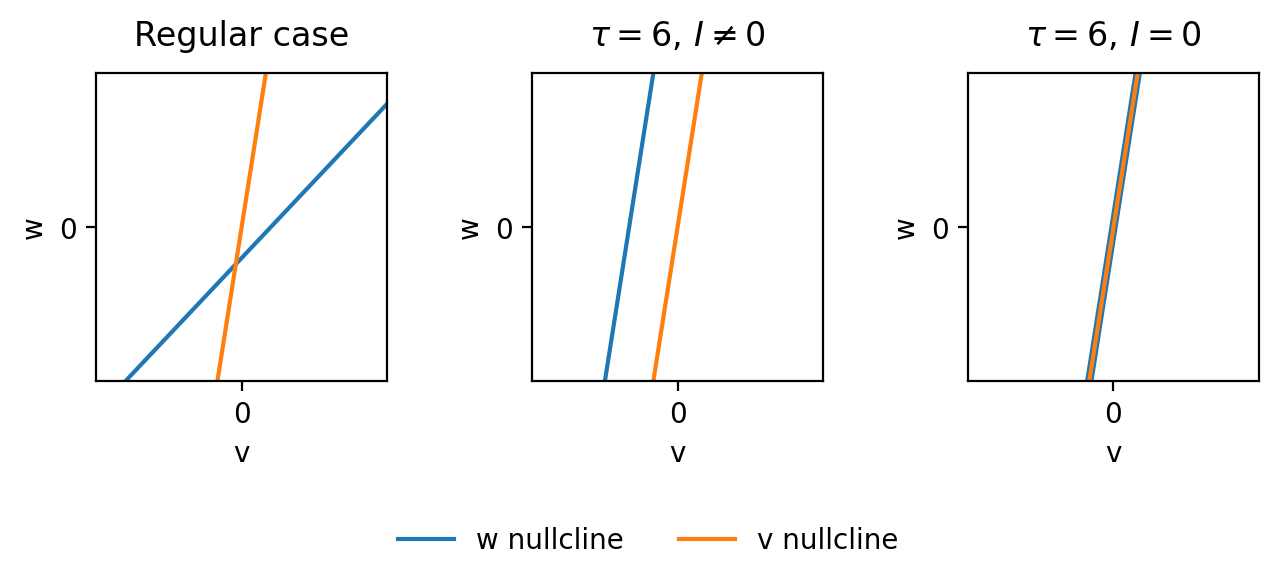
\includegraphics[height=5cm]{nullclines-linear.png}
    \end{figure}

    \item consider the case where $I = 0$. What are the values of $\tau$ for
      which we have only real eigenvalues? What about only imaginary
      eigenvalues?

      We start by solving the characteristic polynomial $P(\lambda)$ associated
      to the system
      %
      \begin{align*}
        &(\lambda - \tau)(\lambda + 2) + 6 = 0\\
        &\lambda^2 + (2-\tau) \lambda + 6 = 0
      \end{align*}
      %
      yielding the following expression for the eigenvalues
      %
      \begin{equation*}
        \lambda_{+/-} = \frac{\tau - 2 \pm \sqrt{(\tau + 2)^2 - 24}}{2}
      \end{equation*}
      %
      The fixed point will have only real eigenvalues when the radicand is
      higher than 0, that is 
      %
      \begin{align*}
        \tau < -\sqrt{24} - 2 \sim -6.8 \quad &or \quad \tau \geq \sqrt{24}-2
        \sim 2.8
      \end{align*}
      %
      Imaginary eigenvalues, on the other hand, require zero real part, which
      can be obtained with $\tau = 2$.

    \item how does the value of $I$ impact the stability of the fixed points?

    It does not impact the stability of the fixed points as it does not appear
    in the system Jacobian. It does, however, impact the coordinate of the fixed
    points by offsetting the $v$ nullcline.

    \textbf{BONUS:} this is also why a linear model is not suitable for neuronal
    modeling: increasing the input current does not lead to spiking, as it
    cannot make the fixed point lose its stability (20 points if they say this).

  \end{enumerate}

  \begin{equation*}
    MSE = \frac{1}{N}\sum_{i}(y_i - ax_i - b)^2
  \end{equation*}

  \begin{equation*}
    y_i = a x_i + b
  \end{equation*}

  \begin{equation*}
    \left\{
    \begin{aligned}
      &\frac{\Delta MSE}{\Delta a} \simeq \frac{\partial MSE}{\partial a} =
      0\\[6pt]
      &\frac{\Delta MSE}{\Delta b} \simeq \frac{\partial MSE}{\partial b} = 0
    \end{aligned} \right. \quad \longrightarrow \quad
    \left\{
    \begin{aligned}
      &a = \frac{\sum_{i}(y_i - \bar{y})(x_i -
      \bar{x})}{\sum_{i}(x_i-\bar{x})^2}\\[6pt]
      &b = \bar{y} - a \bar{x}
    \end{aligned}\right.
  \end{equation*}

  \begin{equation}
    P(\text{spiking}|x) = \frac{1}{1 + e^{-\frac{x - \mu}{s}}}
  \end{equation}
  \begin{equation}
    \mathcal{L} = \sum_{i}l_i, \quad l_i = \left\{
    \begin{aligned}
      &-\log p_i, &&\text{if }y_i = 1\\
      &-\log (1 - p_i), &&\text{if }y_i = 0\\
    \end{aligned}\right.
  \end{equation}

  \begin{equation}
    Y(t) = W_2 \, \sigma(W_1 \, X(t) + b_1) + b_2
  \end{equation}
  % \printbibliography

\end{document}
